\documentclass{beamer}

\usefonttheme{professionalfonts} % using non standard fonts for beamer
\usefonttheme{serif} % default family is serif

\usepackage{hyperref}
%\usepackage{minted}
\usepackage{animate}
\usepackage{graphicx}
\def\Put(#1,#2)#3{\leavevmode\makebox(0,0){\put(#1,#2){#3}}}
\usepackage{colortbl}
\usepackage{tikz}
\usepackage{amssymb}
\usepackage{enumerate}


\newcommand\blfootnote[1]{%

  \begingroup

  \renewcommand\thefootnote{}\footnote{#1}%

  \addtocounter{footnote}{-1}%

  \endgroup

}

\makeatletter

%%%%%%%%%%%%%%%%%%%%%%%%%%%%%% Textclass specific LaTeX commands.

 % this default might be overridden by plain title style

 \newcommand\makebeamertitle{\frame{\maketitle}}%

 % (ERT) argument for the TOC

 \AtBeginDocument{%

   \let\origtableofcontents=\tableofcontents

   \def\tableofcontents{\@ifnextchar[{\origtableofcontents}{\gobbletableofcontents}}

   \def\gobbletableofcontents#1{\origtableofcontents}

 }

%%%%%%%%%%%%%%%%%%%%%%%%%%%%%% User specified LaTeX commands.

\usetheme{Malmoe}

% or ...

\useoutertheme{infolines}

\addtobeamertemplate{headline}{}{\vskip2pt}

\setbeamercovered{transparent}

% or whatever (possibly just delete it)

\makeatother

\begin{document}
\title[PFLOCK report]{PFLOCK Report}
\author[AC]{Andres Calderon}
\institute[Fall'19]{University of California, Riverside}
\makebeamertitle
\newif\iflattersubsect

\AtBeginSection[] {
    \begin{frame}<beamer>
    \frametitle{Outline} 
    \tableofcontents[currentsection]  
    \end{frame}
    \lattersubsectfalse
}

\AtBeginSubsection[] {
    \begin{frame}<beamer>
    \frametitle{Outline} 
    \tableofcontents[currentsubsection]  
    \end{frame}
}

\begin{frame}{Alternative 1}
    \centering
    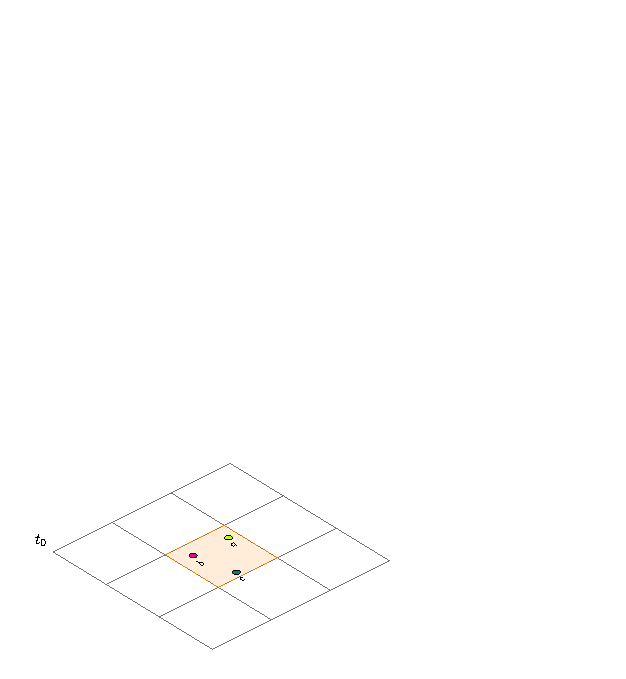
\includegraphics[height=0.95\textheight]{Figures/A1/T0}
\end{frame}
\begin{frame}{Alternative 1}
    \centering
    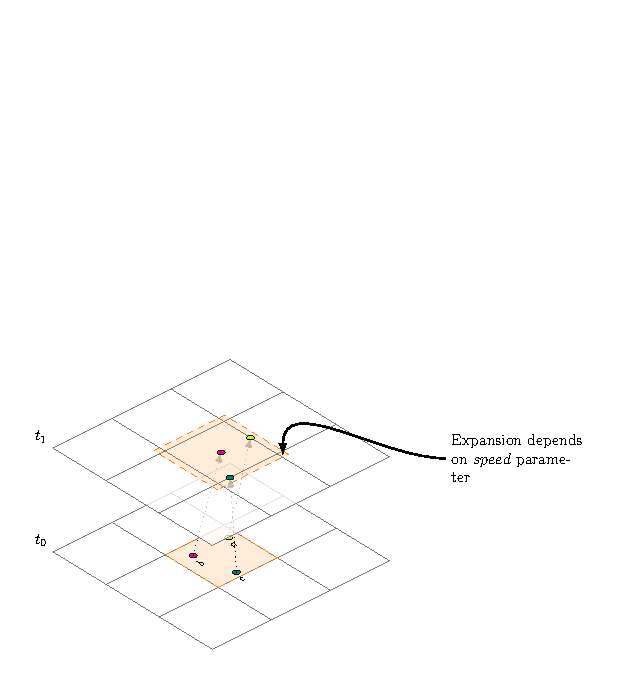
\includegraphics[height=0.95\textheight]{Figures/A1/T1}
\end{frame}
\begin{frame}{Alternative 1}
    \centering
    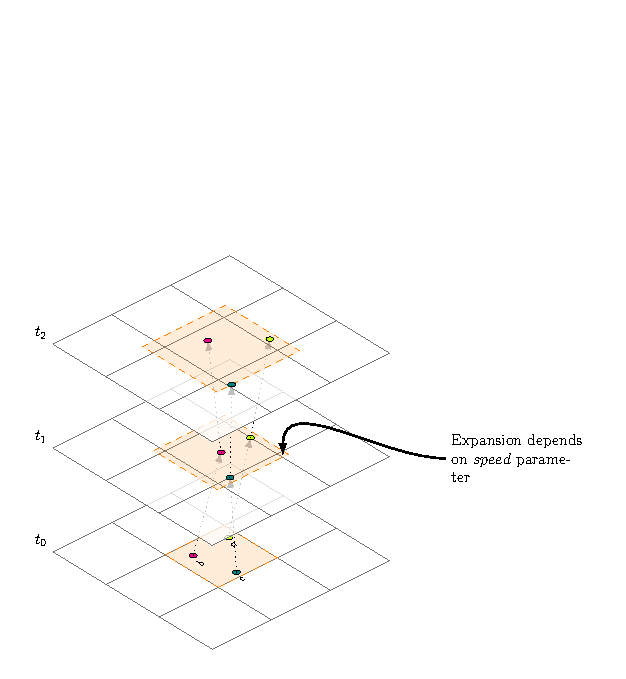
\includegraphics[height=0.95\textheight]{Figures/A1/T2}
\end{frame}
\begin{frame}{Alternative 1}
    \centering
    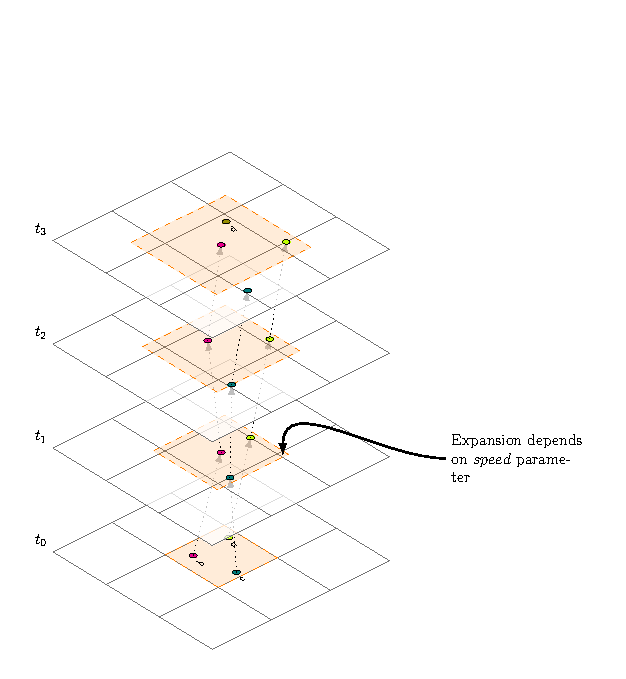
\includegraphics[height=0.95\textheight]{Figures/A1/T3}
\end{frame}
\begin{frame}{Alternative 1}
    \centering
    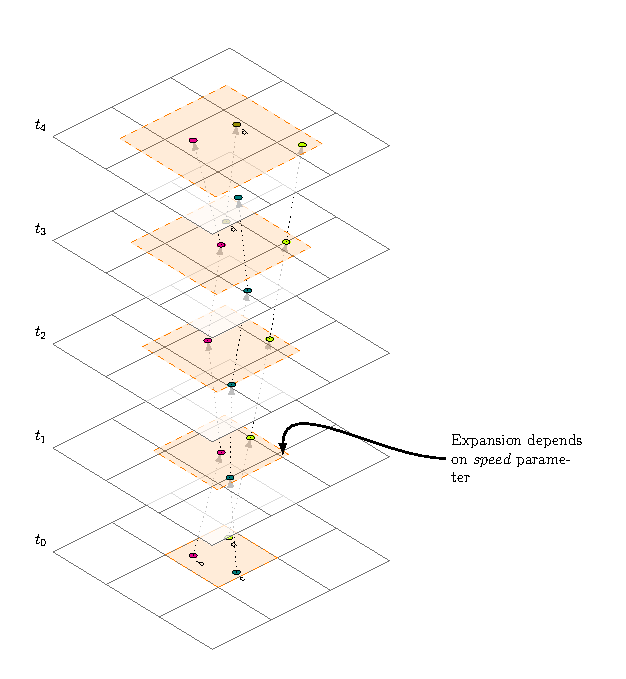
\includegraphics[height=0.95\textheight]{Figures/A1/T4}
\end{frame}

\begin{frame}{Alternative 1}
    \begin{itemize}
        \item Each partition expands according to the \texttt{speed} parameter, so it will have the information of all the trajectories which start on it.
        \item Flocks $a$ and $b$ start in the partition $(1,1)$.  Flock $a$ starts and ends inside of the partition. Flock $b$ leaves the partition but remains inside the expansion area.  Both will be reported.
        \item Flock $c$ starts in the partition $(1,1)$ but leaves the expansion area at time 3.  It will not be reported.
        \item Even flock $d$ starts and end in partition $(1,1)$, it will not be reported because it did not begin at the start of the window (it does not meet the $\delta$ parameter).
    \end{itemize}
\end{frame}


\begin{frame}{Alternative 2}
    \centering
    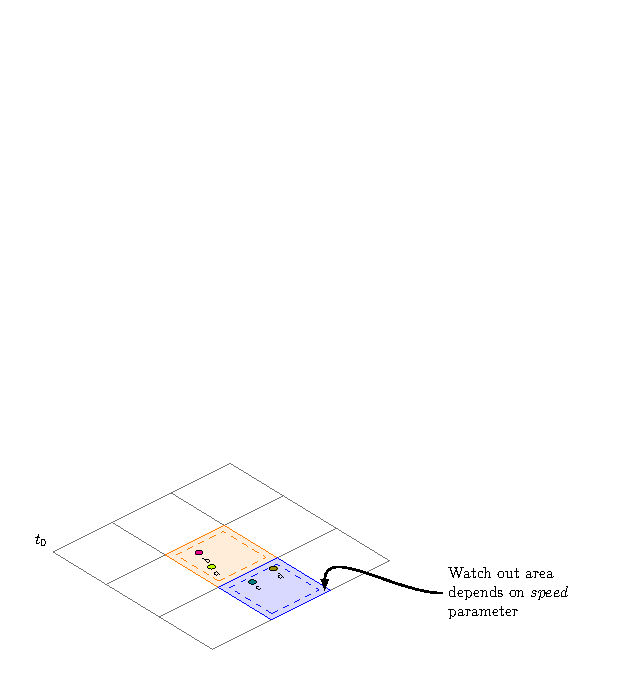
\includegraphics[height=0.95\textheight]{Figures/A2/T0}
\end{frame}
\begin{frame}{Alternative 2}
    \centering
    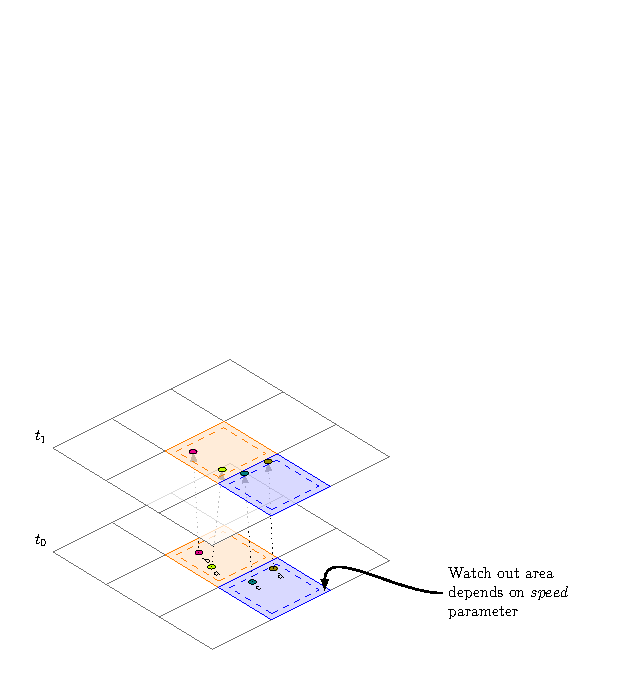
\includegraphics[height=0.95\textheight]{Figures/A2/T1}
\end{frame}
\begin{frame}{Alternative 2}
    \centering
    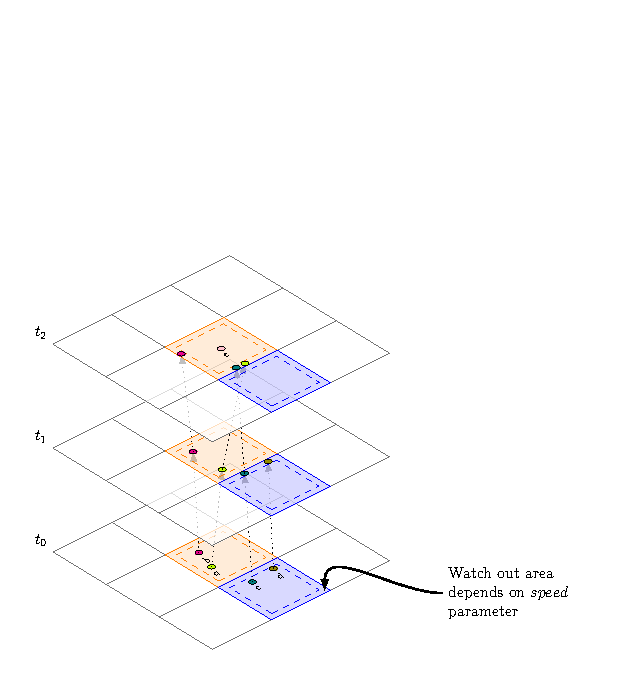
\includegraphics[height=0.95\textheight]{Figures/A2/T2}
\end{frame}
\begin{frame}{Alternative 2}
    \centering
    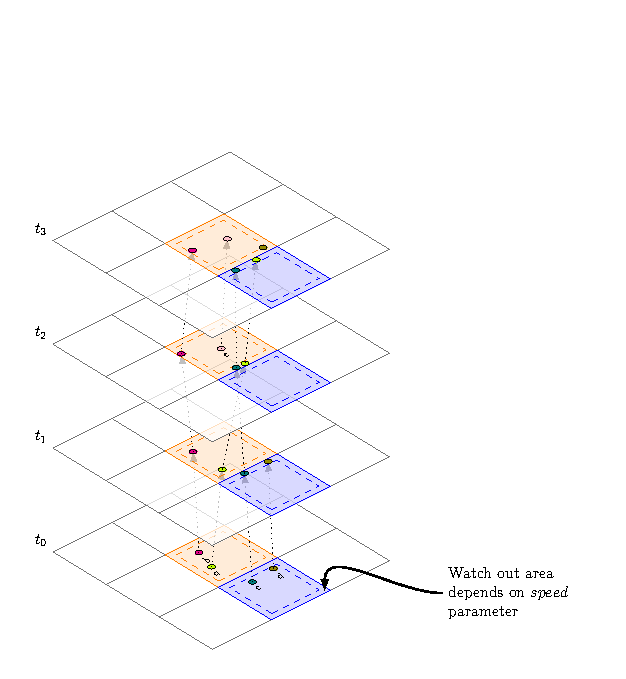
\includegraphics[height=0.95\textheight]{Figures/A2/T3}
\end{frame}
\begin{frame}{Alternative 2}
    \centering
    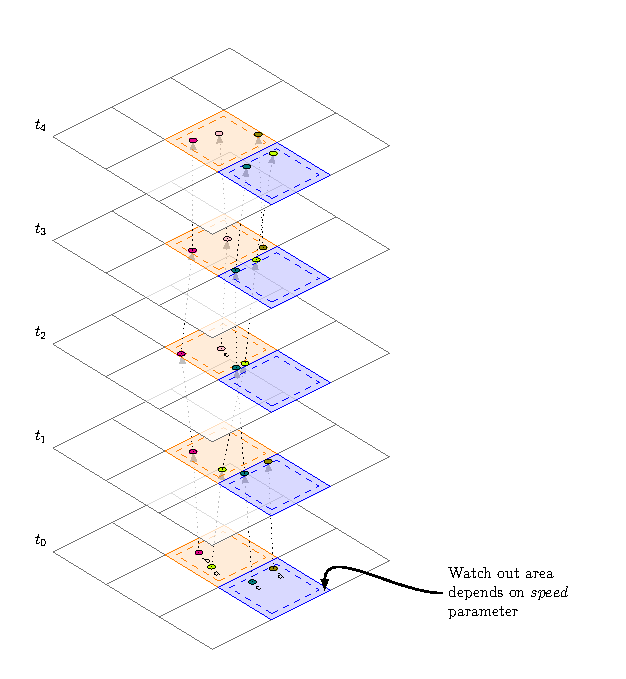
\includegraphics[height=0.95\textheight]{Figures/A2/T4}
\end{frame}

\begin{frame}{Alternative 2}
    \begin{itemize}
        \item Each partition is divided into ``watch out'' and ``safe'' area according to the \texttt{speed} parameter.
        \item Each partition remains fixed and it will report flocks which start and end inside of it if they meet the $\delta$ parameter (i.e. partition $(1,1)$ will report flock $b$ but not flock $e$).
        \item Each partition has to report flocks if they start or end on its ``watch out'' area. They must be post-processed to check it they can be concatenated.  
    \end{itemize}
\end{frame}

\begin{frame}{Alternative 2}
    \begin{itemize}
        \item For example, for flocks $a$, $c$ and $d$ we have:  
    \end{itemize}
    \centering
    \begin{tabular}{ c c c }
        \hline
        Partition (1,1) & Partition (1,0)  & Concat \\
        \hline
        $a_{t_0-t_2}$   & $a_{t_3-t_4}$     & $a_{t_0-t_4}\surd$    \\
        \arrayrulecolor{lightgray}\hline
        $c_{t_2-t_2}$   & $c_{t_0-t_1}$     & $c_{t_0-t_4}\surd$    \\
                        & $c_{t_3-t_4}$     &                       \\
        \hline
        $d_{t_3-t_4}$   & $d_{t_0-t_1}$     & $\times$              \\
        \arrayrulecolor{black}\hline
    \end{tabular}
\end{frame}

\end{document}
